\chapter{Tecnoloxías Empregadas}
    
    O feito de traballar na web, e moito mais o de facelo no ámbito da análise de vídeo, requiren 
    que este sexa un proxecto cuns altos niveis de integración no que toman parte toda unha serie 
    de librerías e ferramentas software que axudan a alcanzar os fins desexado.
    
    Nesta primeiras sección procederase a explicar que tecnoloxías se tiveron en conta á hora de 
    escoller o xeito de implementar este proxecto e con que criterios, para a continuación proceder
    cunha explicación detallada de cada unha de elas. 
    
    \section{Estudo comparativo das tecnoloxías web}
    \label{sec:estudoTecnoloxias}
    Para a elaboración de este traballo de fin de grao, é preciso seleccionar unha serie de
    tecnoloxías tanto para o lado servidor coma para o lado cliente, vamos a empregar os seguintes
    criterios para poder comparalas entre si e escoller entre elas a que mellor se adecúan ás 
    necesidades do proxecto.

    \begin{itemize}

        \item {\textbf{Plataforma e Portabilidade\\}}
            Segundo as especificacións iniciais do proxecto, e de cara a facilitar a 
            implementación deste, as ferramentas empregadas deben de executarse baixo os
            Sistemas Operativos baseados en Linux.

        \item {\textbf{Compatibilidade co algoritmo de Procesado de Vídeo\\}}
            Dado que o algoritmo que procesa o vídeo foi parcialmente implementado en C++,
            a tecnoloxía que se empregue para o desenvolvemento da parte web debe dispoñer da
            máxima compatibilidade con esta linguaxe de programación.

        \item {\textbf{Desenvolvemento Áxil\\}}
            A tecnoloxía que se seleccione ten que minimizar o custe en tempo e esforzo da 
            implementación, por este motivo valorarase positivamente que dispoña de IDE's axeitados,
            facilidades de acceso a BD(Base de Datos),se é posible ORM(Object-Relational Mapping) 
            integrado, recarga en quente... En xeral todo aquelo que permita axilidade e flexibilidade.

    \end{itemize}

    Posto que empregamos unha arquitectura baseada no modelo cliente-servidor, temos que determinar 
    por un lado en que tecnoloxías vamos a construír o Servidor ou Back-End, e por outra parte o 
    Cliente ou Front-End que se executará nun navegador.  

    \subsection{Back-End}
        En canto ás tecnoloxías para a elaboración do Back-End, hai que ter en conta que procesará
        os datos proporcionados polo Front-End, atendendo as súas peticións, e xestionando o modelo de 
        datos e os procesos implicados na aplicación. A maiores neste caso en concreto, o Back-End será
        o encargado de interactuar directamente co sistema de Análise de Vídeo.
        
        As tecnoloxías estudadas para esta parte do sistema son as seguintes:

        \subsubsection{Java}
        Java é unha das linguaxes mais empregadas actualmente. Ademais existen diversos
        frameworks web como Tapestry ou SpringMVC e en canto as BD Hibernate, que facilitan o 
        seu uso, mais é preciso integralos xa que non forman parte da plataforma en si. A súas 
        posibilidades de integración con c++ son altas grazas á interface JNI(Java Native 
        Interface), pero a súa configuración pódese volver tediosa. Un dos proxectos estudados
        para ver o seu funcionamento é Red5 \cite{red5-github-url}.
        
        \subsubsection{C\#}
        Esta linguaxe en combinación con .NET resulta unha combinación bastante áxil de cara
        á programación web, integrando na propia plataforma un deseñador Web e un ORM moi 
        intuitivo. O gran problema polo que se descartou este entorno foi polo seu baixo grao
        de compatibilidade cos sistemas operativos Linux.
        
        \subsubsection{C - C++}
        C++ presenta como era de esperar a maior compatibilidade co algoritmo implementado, non
        obstante, inda que existen algunhas utilidades que facilitan o desenvolvemento web con 
        esta linguaxe como Wt (Web Toolkit)\cite{wt-url}, o grado de axilidade está moi por 
        baixo do que facilitan o resto das combinacións. Tamén pode resultar de interese o
        coñecido proxecto Icecast\cite{icecast-url}, que fai streaming de vídeo sobre unha 
        interface web.
        
        \subsubsection{Python + Django}
        Python presentase como a mellor opción para desenvolver o lado servidor, por unha parte
        dispón do módulo Subprocess\cite{subprocess-module-url} que permite executar calquera
        comando pola terminal maximizando así a modularidade e a integración co algoritmo en C++.
        Por outra parte Django\cite{django-web-page-url} contén un potente ORM e un sistema de 
        "Templates" que simplifica a parte web. Para concluír cabe destacar o feito de que 
        python sexa unha linguaxe interpretada, xa que isto evita o paso previo de compilación.
        
        
    \subsection{Front-End}
        Unha vez seleccionada a tecnoloxía do lado servidor, é hora de ver que opcións existen para
        o Front-End, a parte do Sistema encargada da interacción co usuario.
        
        Por unha parte están as tecnoloxías que pola súa transcendencia e nivel de aceptación
        cosideranse xa imprescindibles no desenvolvemento web, estamos a falar de HTML e CSS linguaxes
        de facto para definir o contido e o aspecto visual respectivamente dunha páxina web.
        De estas linguaxes seleccionaremos as súas versións mais recentes, que a día de hoxe son HTML5 e
        CSS3.
        
        Sen embargo, noutros campos coma son a reprodución de vídeo e o control de elementos dinámicos
        non existe unha tecnoloxía que abarque a case completitude da rede, é por elo que neste capítulo
        estudaremos aqueles xeitos que permitan a reprodución de vídeo e a maiores o debuxado de 
        figuras en movemento sobre este vídeo.\\
        
        En canto á reprodución de vídeo e o control deste destacan principalmente dúas alternativas:
        
        \subsubsection{Vídeo en Flash}
            Vídeo Flash é a tecnoloxía de reprodución de vídeo mais empregada e madura en
            internet dende hai anos. Inicialmente creada por Macromedia e mercada por Adobe 
            en 2005, permite crear elaboradas animacións vectoriais, que logo poden proxectarse
            sobre un vídeo, mentres que tamén manexa os eventos de reprodución de vídeo como o 
            play ou o stop.\\
            
            Ten certos problemas en tanto ao Posicionamento Web(SEO), reprodución en 
            dispositivos móbiles, accesibilidade... pero o meirande de todos eles é que mentres
            que outros dos exemplos estudados son 100\% libres, Flash é un programa propietario
            para o que é preciso adquirir unha licencia.        
            
        
        \subsubsection{Vídeo HTML5 + Javascript}
            Esta é outra das combinacións mais empregadas actualmente, xa que segue o estándar
            do W3C (World Wide Web Consortium)\cite{w3schools-video-tag} no que se defíne como se
            han de mostrar e obter os vídeos dunha páxina codificada coa linguaxe HTML5., e 
            destaca por seres extremadamente sinxelo en comparación con Flash ou outras tecnoloxías.
            
            Se o comparamos con Flash podemos ver a seguintes \textbf{vantaxes:}
            \begin{itemize}
                \item Resulta moito mais sinxelo de codificar grazas a que é o navegador o que se 
                encarga da reprodución do vídeo mentres que o programador só define o xeito de obtelo.
                \item Non precisa da instalación de ningún Plugin que poida dar problemas por exemplo 
                en dispositivos móbiles.
                \item Mentres que HTML5 e Javascript son libres, Flash é unha tecnoloxía propiedade de 
                Adobe.
                \item HTML5 + CSS3 dispón de mais facilidades se buscamos un deseño ``responsive''.
            \end{itemize}

            Será por tanto a alternativa escollida para a construción deste proxecto, e en canto ao 
            debuxo de figuras sobre o vídeo escolleremos o elemento $<canvas>$ tamén de HTML5. Todas
            estas tecnoloxías e moitas mais explícanse en detalle no seguinte capítulo.
            
    
    %%%%%%%%%%%%%%%%%%%%%%%%%%%%%%%%%%%%%%%%%%%%%%%%%%%%%%%%%%%%%%%%%%%%%%%%%%%%%%%%%%%%%%%%%%%%%%%
    
    
    A continuación explicase detidamente cal é a función de cada unha das tecnoloxías que forman 
    parte deste proxecto co fin de comprender o explicado nos capítulos seguintes. O diagrama 
    \ref{fig:ArqSistemaCustom} pode servir como orientación á hora de comprender que función 
    desempeña cada unha de elas.
    
    \begin{figure}[htp]
    \begin{center}
        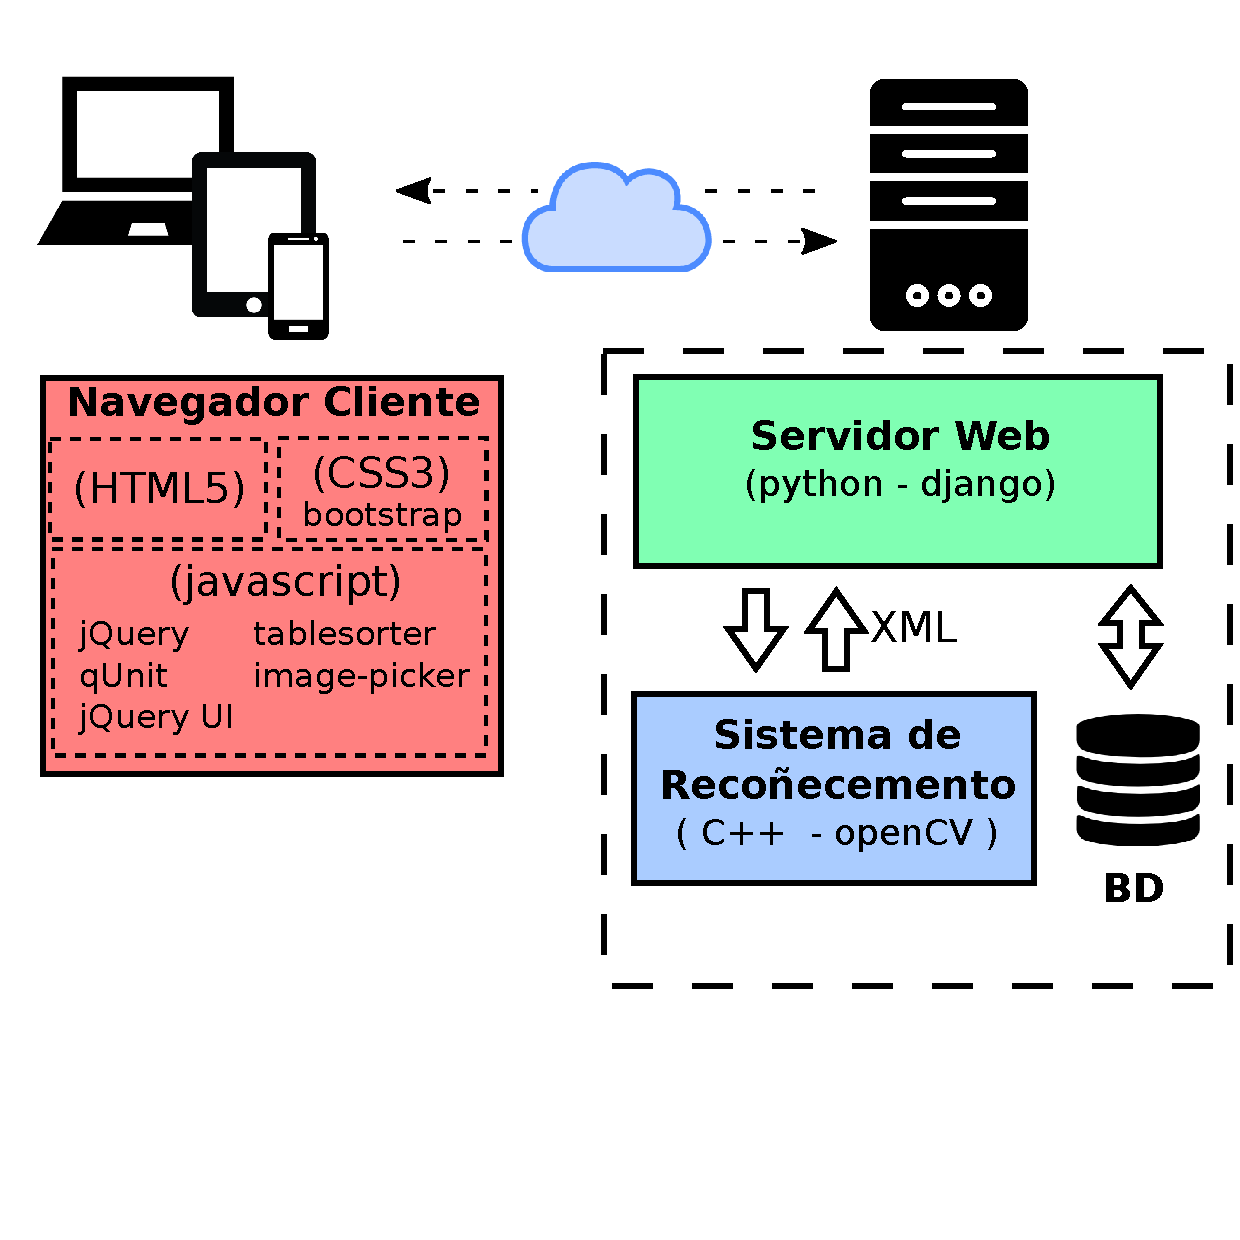
\includegraphics[scale=0.6]{figures/ArqSistemaCustom.pdf}
        \caption{Diagrama da Arquitectura do Sistema}
    \label{fig:ArqSistemaCustom}
    \end{center}
    \end{figure}
    
    Comezamos polas tecnoloxías empregadas no lado cliente:
    \section{Navegador Ciente}
    
    O navegador do cliente empregará unha serie de tecnoloxías para mostrar os datos obtidos do 
    servidor, as mais destacables son:
    
    \subsection{HTML5}
        HTML (HyperText Markup Language) é a linguaxe de marcas empregada en internet para a elaboración
        de páxinas web, define unha estrutura básica e un código para a definición do contido da páxina
        como poden ser texto, imaxes, vídeos... Existen diversas versións deste estándar, mais para este
        proxecto empregarase a sua última versión HTML5, que inclúe toda unha serie de novos elementos.
        
        Un dos compoñentes que mais empregaremos para a construción desta web será o elemento 
        $<video>$ de HTML5 que achega unha serie de Métodos, Eventos e Propiedades
        \cite{w3school-video-events} que poden empregarse dende o código Javascript.
        
        A maiores do propio contido da páxina, HTML permite incluír referencias a outros ficheiros que 
        están tamén asociados á páxina como poden ser ficheiros javascript ou css que se mostran de 
        seguido.
    
    \subsection{CSS3}
        HTML permite unha perfecta estruturación dos elementos que compoñen unha páxina web, pero 
        en caso de que queiramos personalizar o estilo da páxina web, ou adaptala a diferentes 
        dispositivos precisamos CSS. CSS(Cascading Style Sheets) é unha linguaxe para definir e 
        crear a presentación dun documento HTML.
        
        Para elo defínense unha ou mais follas de estilos, que definen para cada elemento 
        seleccionado nelas unha serie de características de estilo. No caso da aplicación a 
        desenvolver a política de follas de estilo será a de crear unha folla de estilo xeral para 
        conter as características de estilo comúns a todo o proxecto e a maiores as que sexan 
        precisas para páxinas ou elementos concretos, todo elo traballando coa versión 3 desta linguaxe.
    
        Por sorte, para simplificar o traballo na definición do estilo xeral da páxina existen 
        librerías CSS como bootstrap que definen parte do código preciso, isto dá un estilo 
        uniforme á web ao tempo que axuda a reducir o tempo de implementación.
        
        \subsubsection{Twitter Bootstrap}
            Twitter bootstrap é un framework ou conxunto de ferramentas de código aberto para 
            deseñar webs. Contén todo un conxunto de platillas como tipografía, botons, formularios,
            táboas, barras de navegación... Estas plantillas normalmente consisten simplemente nun
            estilo CSS, pero ás veces tamén hai un procesado en javascript como o da función popover
            que permite xerar unha ventá flotante para amosar os datos dos obxectos detectados na 
            aplicación.
            
            A pesar de todas as cousas que permiten facer HTML + CSS moitas veces é preciso un 
            tratamento dinámico da información e neste caso é preciso o emprego dunha linguaxe de 
            scripting como javascript.
    
    \subsection{Javascrpit}
        Javascript é a linguaxe de programación interpretada que se executa nos navegadores
        cumprindo co estándar ECMAScript, permite executar ordes podendo interactuar coa páxina 
        web a través da arbore DOM (Document Object Model) e co servidor mediante o sistema de
        chamadas asíncronas. Cada scrpit en javascript está asociado a unha páxina web, de forma
        que todo o que executemos terá efecto sobre a páxina actual e nunca poderemos prolongar
        a execución dun código .js mais aló da vida desta páxina.\\
        
        A pesar de executarse nun navegador javascript é unha linguaxe cunha potencia 
        considerable, esta potencia ven da súa orientación a obxectos que tamén permite 
        programación imperativa con un tipado débil e dinámico.\\
        
        Javascript pode incluírse directamente no documento HTML, mais isto é problemático 
        porque mestura dúas linguaxes e non permite a reutilización do código javascript en
        distintas páxinas, polo que na practica sempre se traballará con código contido en
        ficheiros .js que logo serán importados dende as páxinas web que o precisen. Mediante 
        referencias tamén se pode engadir código de librarías, que pode achegarse de dous xeitos
        distintos, ou ben cun enlace á páxina onde están publicadas, ou ben descargando estas
        librerías ao servidor da aplicación e ofrecéndoas dende aí. O enfoque seguido neste 
        proxecto é o segundo, pois de este xeito a aplicación está auto-contida, podendo traballar
        sen conexión con internet, e mantendo sempre a integridade a pesar de que o provedor
        da biblioteca decida deixar de ofrecela.\\
        
        Mediante Javascript tamén pode manexarse o elemento $<canvas>$ de HTML5, que xera un mapa
        de bits para construír gráficos, manipular imaxes e crear dinamicamente animacións nunha
        páxina web. A única dúbida que soe xurdir sobre esta tecnoloxía está en canto ao seu 
        rendemento e alcance, pero exemplos como os que amosa Kevin Roast na súa páxina 
        web\cite{kevin-roast-canvas-examples} despexan toda dúbida posíbel.\\
        
        Por desgraza, a execución en navegador ten tamén os seus inconvintes como a execución 
        multi-threading empregando \textbf{Web Workers}, estes elementos pensados para permitir
        a execución paralela de código javascript deixan polo de agora moito que desexar xa que 
        cada thread ten as súas propias variables estancas, impedindo polo tanto o acceso á 
        arbore DOM dende threads paralelos co problema engadido de que algúns navegadores como 
        Opera en vez de facer un multi-threading sobre threads do propio sistema  tan só simulan
        este fenómeno nun único thread. O paralelismo cobrará especial importancia 
        cando executemos os algoritmos que mostran os datos da análise en XML, pois ao 
        executarse todo no mesmo fio debemos prestar especial atención a non bloquear a 
        interface de usuario con tarefas moi prolongadas.\\
    
        Javascript tamén é especialmente potente e sinxelo á hora de parsear documentos, xa sexa
        un documento HTML para acceder á arbore DOM ou ben un XML como o que xera o sistema de 
        análise. Por desgraza, o manexo de excepcións, e as veces a selección de elementos dentro de un 
        documento poden ser tarefas tediosas con javascript, co fin de simplificar isto empregaremos
        a biblioteca jQuery.
            
        \subsubsection{jQuery}
        
            jQuery é unha biblioteca javascript pensada para simplificar os aspectos mais complexos desta 
            linguaxe como poden ser a manipulación de documentos HTML/XML ou as chamadas asíncronas 
            mediante AJAX. Está escrita en javascript e é 100\% libre, tal vez por isto sexa a biblioteca
            javascript mais empregada.
            
            O sistema de selección de jQuery é o mesmo que se emprega en CSS, permitindo seleccionar de 
            xeito sinxelo un conxunto de elementos dentro dun documento, a maiores tamén dispón de un 
            sinxelo acceso e modificación tantos destes elementos como dos seus atributos.
            
            Os mesmos autores de jQuery, en vista de que no mundo javascript existían outros moitos
            aspectos a simplificar decidiron outras bibliotecas como as que se amosan a continuación:
            
        \subsubsection{Qunit}
        
            QUnit é un framework de probas unitarias para código javascript doado de empregar e bastante
            poderoso. Empregase tanto en jQuery, jQuery UI e os proxectos de jQuery Mobile sendo capaz 
            de probar calquera código javascript xenérico.
            
            Para facer probas emprega un conxunto de sentencias assert como todas as bibliotecas que 
            realizan tests de unidade. No caso da nosa aplicación empregarase para probar todo aquel
            código independente da arbore DOM da páxina. É importante destacar que co fin de maximizar
            a facilidade de proba do código na capa javascript seguíronse os consellos amosados na páxina
            de Qunit\cite{QunitMakeItTesteable} e unha interpretación flexible do MVC(Modelo 
            Vista Controlador) onde a vista está conformada polo código HTML+CSS, o controlador polo 
            manexadores dos ficheiros video-player.js, video-controls.js e por último as clases do 
            modelo en javascript nos ficheiros Detection.js, DetectionObserver.js, VideoDetections.js e 
            en menor medida suspicious-popup.js.
        
        \subsubsection{Image-picker}
        
            Outra librería tamén baseada en jQuery é Image-Picker \cite{ImagePickerPage} que permite
            xerar un formulario cun campo de tipo ``select'' baseado en imaxes en vez de nunha 
            entrada despregable, todo elo de forma extremadamente sinxela.
        
        \subsubsection{jQuery UI}
        
            jQuery UI é unha biblioteca de compoñentes para jQuery que lle engade un conxunto de 
            plugins, widgets e efectos visuais. Pódese descargar dende a súa páxina oficial o 
            nucleo da biblioteca e os compoñentes nos que se estea interesado, que no caso deste
            proxecto  empregase o compoñente slider\cite{ComponenteSliderJqueryUi} que
            xera unha barra selectora.
        
        \subsubsection{tablesorter}
        
            A derradeira biblioteca empregada, tamén baseada en jQuery é tablesorter
            \cite{tablesorter-webPage}. Tablesorter é un plugin baseado en jQuery para transformar 
            unha táboa HTML estándar coas etiquetas $<thead>$ e $<tbody>$ nunha táboa que se pode 
            ordenar polo contido das distintas columnas sen ter que recarga-la páxina. Neste
            caso será de moita utilidade á hora de amosar os resultados da análise, pois así 
            poderanse ordenar as deteccións segundo aparecen no vídeo, segundo o tempo que pasan 
            en pantalla... 
        
    Todas estas tecnoloxías de capa web axudarannos a mostrar con mais facilidade a análise que o
    sistema de recoñecemento faga do vídeo, e en canto as ferramentas empregadas para esta análise
    a ferramenta fundamental que se empregará é OpenCV.
    
\section{Sistema de Recoñecemento}
    O sistema de recoñecemento debe ser capaz de ler un vídeo e en base a el recoñecer os obxectos
    de ese vídeo á vez que analiza o seu comportamento. Isto pódese implementar de distintos xeitos,
    mais neste proxecto en concreto fíxose empregando a linguaxe de programación C++ que xa se citou
    na sección \ref{sec:estudoTecnoloxias}, en combinación coa librería OpenCV e a lingaxe de marcas
    XML.

\subsection{OpenCV}
    
    OpenCV é unha biblioteca libre de visión artificial escrita en código C/C++ optimizado.
    Dende a súa aparición publicada por Intel en Xaneiro de 1999, empregouse en infinidade 
    de proxectos, tanto para detección de movemento como para aplicativos de control de procesos
    que requiren recoñecemento de obxectos.
    
    OpenCV é multiplataforma, existindo versión para GNU/Linux, Mac OS X e Windows. Contén mais 
    de 500 funcións que abarcan unha ampla gama de áreas como o proceso de visión, recoñecemento
    de obxectos (tamén recoñecemento facial), calibrado de cámaras, realidade aumentada e visión
    robótica.
    
    Por todas estas características OpenCV é unha das bibliotecas mais empregadas hoxe en día, e é
    por elo tamén que se escolleu para a implementación do sistema de recoñecemento que a aplicación
    web empregará para a análise do vídeo.
    
    Non obstante, xa que se desexa que a aplicación web sexa o mais versátil posible, contemplase a
    posibilidade de que poida empregar para a análise sistemas desenvoltos noutras tecnoloxías como
    pode ser Matlab. E para dotala deste grao de versatilidade decídese definir unha interface de
    liña de comando a través da cal se chamará ao sistema, e un formato de ficheiro XML (Extensible 
    Markup Language) no que este sistema de recoñecemento deben escribir os datos da súa análise.
        
\subsection{Extensible Markup Language (XML)}
    XML é unha linguaxe de marcas desenvolvida polo W3C (World Wide Web Consortium) e empregado
    para almacenar datos de forma clara e lexible. Permite definir a gramática de linguaxes 
    específicas para estruturar así grandes documentos.
    
    Os documentos XML seguen una estrutura xerárquica baseada en etiquetas(tag's) e atributos,
    que se poden definir nunha Definición de Tipo de Documento ou DTD. \cite{dtd-web-page}
    
    Cando un documento en formato XML segue as directrices definidas no ficheiro DTD asociado,
    dise que este ficheiro esta ben formado(well formed en ingles), e para validar iso empregarase
    na elaboración do traballo algún avaliador de XML en liña como por exemplo o da W3Chools.\cite{xml-validator}
    
    XML é especialmente útil para comunicar varias aplicacións que traballan en tecnoloxías 
    diferentes grazas á súa simplicidade que permite integrar os datos de xeito moi sinxelo. Precisamente
    por iso, servirá como nexo de unión entre o sistema de análise e a aplicación web. 
    
    Para a modificación da súa aparencia pódese empregar \emph{CSS3} (Follas de Estilos en 
    Cascada), e para modificar o seu comportamento, o elemento $<video>$ de HTML5 achega
    unha serie de Métodos, Eventos e Propiedades\cite{w3school-video-events} que poden
    empregarse dende código \emph{Javascript}.
    
\section{Servidor Web}
    Como se explicou anteriormente na sección \ref{sec:estudoTecnoloxias} Django é un framework
    que traballa sobre python para a creación de páxinas web, as súas funcionalidades empregadas
    explicaranse pouco a pouco no capítulo \ref{cap:desenvolvemento}, polo que aquí explicaranse
    outros compoñentes do servidor empregados que compre coñecer antes de proseguir, en concreto 
    ffmpeg.
    
\subsection{FFmpeg}
    Falaremos por tanto de FFmpeg, o software que se empregará no proxecto tanto para obter 
    distinta información de un vídeo como para convertelo a diferentes formatos, unha colección de 
    software libre que pode gravar, converter (transcodificar) e facer streaming de audio e vídeo,
    nel está incluído libavcodec unha biblioteca de codecs que contén aqueles mais empregados.
    
    FFmpeg é un programa bastante sinxelo a pesar do seu grandioso abanico de opcións, no referente
    ao proxecto, emprégao a aplicación web para facer diferentes tarefas como obter un determinado
    fotograma dentro dun vídeo, cambiar o formato no que se almacena ou obter a súa información como
    duración, numero de fotogramas por segundo, etc.
    